\documentclass[fleqn]{article}


\usepackage{pgfplots}
\usepackage{mathexam}
\usepackage{amsmath}
\usepackage{amsfonts}
\usepackage{graphicx}
\usepackage{wrapfig}
\usepackage{systeme}
\usepackage{microtype}
\usepackage{multirow}
\usepackage{pgfplots}
\usepackage{listings}
\usepackage{tikz}
\usepackage{dsfont} %Numeros reales, naturales...
\usepackage{cancel}
\usepackage{verbatim} %comentarios de parrafos

%\graphicspath{{images/}}
\newcommand*{\QED}{\hfill\ensuremath{\square}}

%Estructura de ecuaciones
\setlength{\textwidth}{15cm} \setlength{\oddsidemargin}{5mm}
\setlength{\textheight}{23cm} \setlength{\topmargin}{-1cm}



\author{David García Curbelo}
\title{Topología}

\pagestyle{empty}


\def\R{\mathds{R}}
\def\Z{\mathds{Z}}
\def\N{\mathds{N}}
\def\S{\mathds{S}}

\def\sup{$^2$}

\def\next{\quad \Rightarrow \quad}

\begin{document}

    \setcounter{page}{1}
    \pagestyle{plain}

    \begin{center}
        {\large\bf{Topología II}} \\
        \bf{David García Curbelo}\\
        
    \end{center}

    \textbf{Ejercicio 13.b). } \textit{Para la siguiente presentación de superficie, calcula la caracteríastica de Euler y determina a 
                    cual de las superficies modelo es homeomorfa:}
                    
                    \begin{center}
                        {\Large{$<a,b,c; abca^{-1}b^{-1}c^{-1}>$}}
                    \end{center}


    Consideremos La presentación poligonal de nuestra superficie:
    \begin{wrapfigure}{l}{0.4\textwidth}
        \centering
        \includegraphics[width=0.3\textwidth]{presentación.png}
    \end{wrapfigure}

    
    Veamos cuántos vértices tiene nuestra presentación. Tomemos por $v_1$ al vértice final del lado $a$ de nuestra palabra. Dicho vértice ha de estar
    identificado con el vértice final del lado $a^{-1}$, el cual es fácil observar que coincide con el vértice final del lado $c$. Este a su vez 
    ha de estar identificado con el final de su inverso, el $c^{-1}$. Al estar conectados el final del lado $c^{-1}$ con el principio del lado $b^{-1}$,
    éste forzosamente ha de estar identificado de igual manera con el principio del lado $b$, que al ser el mismo que el vértice del final de $a$, 
    que sabemos que es $v_1$, tenemos completametne localizado nuestro vértice $v_1$ en nuestra superficie. Ilustramos este proceso gráficamente:

    \begin{center}
        \noindent
        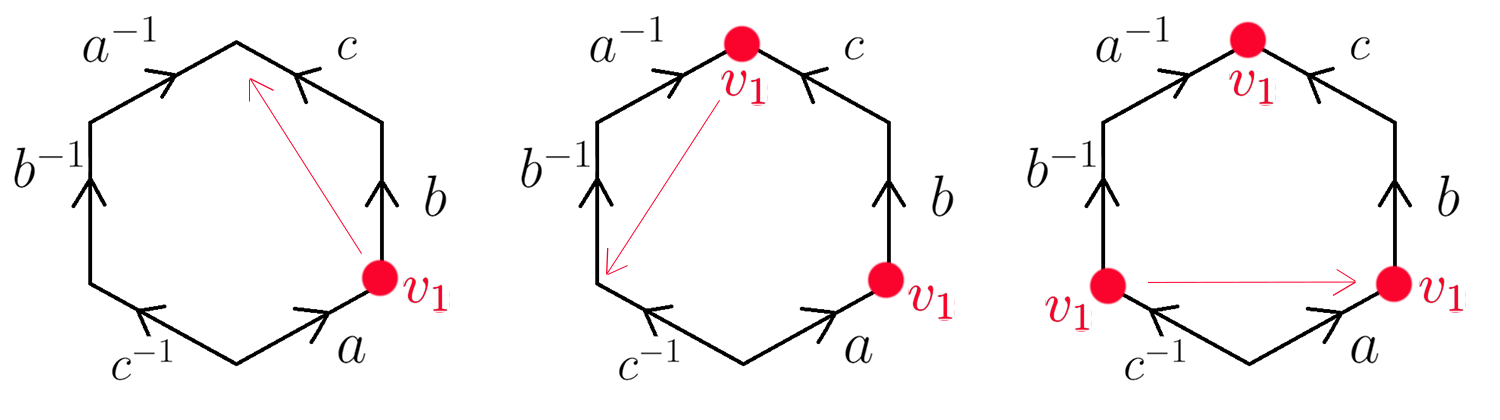
\includegraphics[width=1\linewidth]{v1.png}    
    \end{center}

    Realizamos ahora el mismo proceso para $v_2$. Consideremos como punto de partida el inicio del lado $a$. Este, al ser adyacente con el inicio 
    de $c^{-1}$, estará identificado con el inicio del lado $c$. Vemos que dicho vértice conecta $c$ con el final del lado $b$, luego dicho vértice 
    también identifica con el final de $b^{-1}$, y de la misma manera, al ser adyacente con el principio del inverso de $a$, volvemos al vértice $v_2$
    que habíamos definido en un principio, y por tanto dicho vértice queda totalmente identificado. 
    
    \begin{center}
        \noindent
        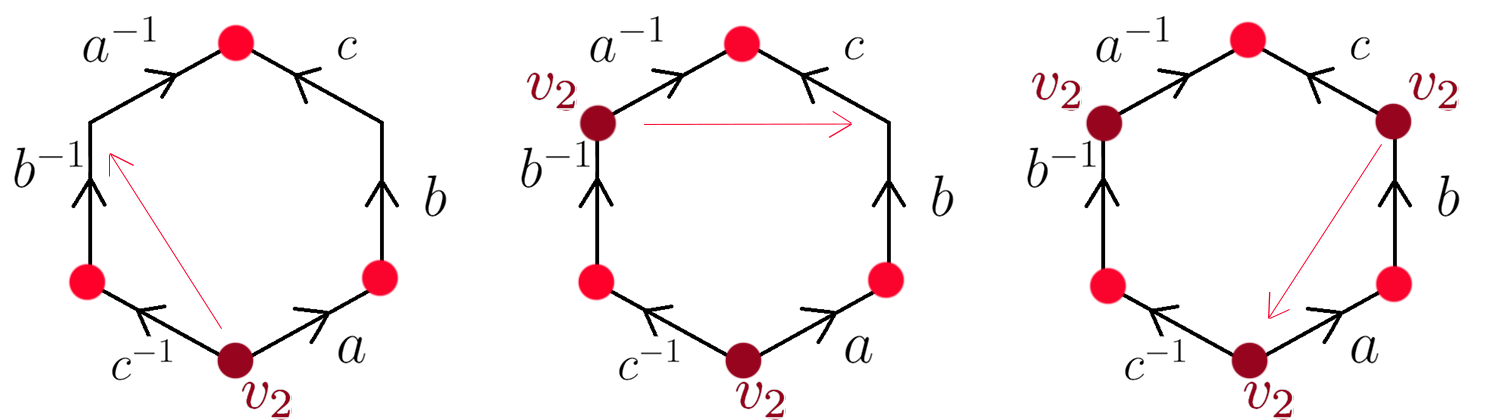
\includegraphics[width=1\linewidth]{v2.png}    
    \end{center}

    Con esta información ya estamos preparados para clasificar nuestra superficie. Como podemos ver, no ha quedado ningún vértice sin identificar, y 
    el número de vértices que hemos requerido ha sido 2. Además, nuestra superficie está conformada por una sola palabra, la cual tiene tres aristas
    distintas. Siendo todo esto así, y ayudándonos de la característica de Euler podemos ver que la característica de Euler de nuestra superficie es 
    $$\chi(P) = C - A + V = 1 - 3 + 2 = 0 $$

    Sabemos que nuestra superficie debe ser homeomorfa a alguna de las superficies modelos. Ya que $\chi(P) = 0$ es par, nos encontramos ante el conflicto
    de no saber si nuestra superficie es un Toro o la suma conexa de dos planos proyectivos. Para ello consideremos de nuevo palabra de nuestra presentación,
    y apliquémosle transformaciones elementales para poder estudiar su orientabilidad (que no tenga aristas retorcidas):
    $$abca^{-1}b^{-1}c^{-1} \overset{Rotar}{\approx} bca^{-1}b^{-1}c^{-1}a \overset{Consolidar}{\approx} bxb^{-1}x^{-1} \overset{Renombrar}{\approx} aba^{-1}b^{-1}$$

    Vemos así claramente que nuestra superficie dada por la presentación $<a,b,c; abca^{-1}b^{-1}c^{-1}>$ es orientable por no presentar aristas retorcidas, 
    luego ha de ser homeomorfa a un Toro.
\end{document}
